\documentclass[a4paper,10pt]{article}
\usepackage{a4wide, graphicx, fancyhdr, amssymb, alg, modalg, wrapfig, amsmath, listings, ifthen, longtable, hanging, enumitem, tabto, float, caption,  tabto, epstopdf, tocloft, lastpage}
\usepackage[usenames,dvipsnames]{color}
\usepackage[left=1.3cm,right=1.3cm,top=2.0cm,bottom=0.8cm]{geometry}
\usepackage{multicol}
\usepackage[toc]{multitoc}
%\usepackage{inconsolata}
\usepackage[calcwidth]{titlesec}
\usepackage[hidelinks]{hyperref}

% \topmargin -2.7cm
%\leftmargin -1.51cm


%------------------------- 
% Colors 
%-------------------------
\definecolor{BrightBlue}{rgb}{0,0,1}
\definecolor{LightGray}{gray}{0.90}
%------------------------- 
% Listings settings 
%-------------------------
\lstset{
    language=java,
    basicstyle=\fontsize{9}{11}\ttfamily,
    keywordstyle=\color{Black},%BrightBlue
%    identifierstyle=\ttfamily,
    commentstyle=\color{Gray},%Green
    stringstyle=\color{Black},%Gray
    showstringspaces=false,
    moreemph={[9]__multiple_inheritance,__single_inheritance,__virtual_inheritance,
                 catch,class,const_cast,
                 delete,dynamic_cast,
                 explicit,export,
                 false,friend,
                 inline,
                 mutable,
                 namespace,new,
                 operator,
                 private,protected,public,
                 reinterpret_cast,
                 static_cast,
                 template,this,throw,true,try,typeid,typename,
                 using,
                 virtual,
                 wchar_t},   % Ultraedit STYLE_KEYWORD
    emphstyle={[9]\color{Black}},%Red
    numbers=left,
    numberstyle=\tiny,
    stepnumber=1,
    numbersep=5pt,
%    frameround=tttt,
    frame=single,
    rulecolor=\color{Black}, %Gray
    columns=fixed,
    xleftmargin=1.5em, % needs to compensate for the frame margin
%    xrightmargin=3em,
%    framexleftmargin=1.5em,
    tabsize=2,
    breaklines=true
}

%----------------------- 
% Macros and Definitions 
% ----------------------
\newcommand{\N}{\mathbb{N}}
\newcommand{\Z}{\mathbb{Z}}
\titlespacing*{\section}{0pt}{0.2\baselineskip}{0.2\baselineskip}
\titlespacing*{\subsection}{0pt}{0.5\baselineskip}{0.2\baselineskip}
\titlespacing*{\subsubsection}{0pt}{0.15\baselineskip}{0.15\baselineskip}
\setlength{\cftbeforesecskip}{0pt}
\setlist[itemize]{leftmargin=13pt}
\setlist[enumerate]{leftmargin=13pt}
\NumTabs{12}
\renewcommand{\contentsname}{Contents\vspace{-8pt}}
%--------------------
% Page style settings
%--------------------
\renewcommand*{\multicolumntoc}{2}
\setlength{\columnseprule}{0pt}
\setlength{\headsep}{0.25cm}
%\setlength\headheight{20pt}
%\addtolength\topmargin{-10pt}

\fancypagestyle{plain}{%
\fancyhf{}
\fancyhead[L]{\sffamily\bfseries Eindhoven University of Technology}
\fancyhead[R]{\sffamily\bfseries{\thepage/\pageref{LastPage}}}
\renewcommand{\headrulewidth}{1pt}
\renewcommand{\footrulewidth}{0pt}
}



\pagestyle{fancy}
\fancyhf{}
\fancyhead[L]{\sffamily\bfseries Eindhoven University of Technology}
\fancyhead[R]{\sffamily\bfseries{\thepage/\pageref{LastPage}}}
\renewcommand{\headrulewidth}{1pt}
\renewcommand{\footrulewidth}{0pt}

\graphicspath{{figures/}}

%-----------------
% Title 
%-----------------
\title{\vspace{-1cm}\textmd{\textbf{Team 386491}}\\\vspace{5pt}\Large\textbf{{Cheatsheet for SOMERANDOMCONTEST}}\\\vspace{5pt}\large{Frank Maurix\hspace{1.5cm} Patrick Shaw\hspace{1.5cm} Luca Weibel}}
\author{}\date{}

%-----------------
% Start of document
%-----------------
\begin{document}
\maketitle
\vspace{-2.1cm}
\tableofcontents


\newpage\section{General Stuff}
\subsection{Running times}
$\begin{array}{lll}
\mbox{\textbf{Value}} & \mbox{\textbf{Possible running times}} & \mbox{\textbf{Which algorithms to use?}} \\
n \leq 10^9 & O(1), O(\log( n)), O(\sqrt{n}) & \mbox{Function, Binary Search} \\
n \leq 10^6 & O(n), O(n \cdot\log( n)) & \mbox{Greedy, sorting, Binary Search + Greedy, Divide and Conquer} \\
n \leq 10^3, W \leq 10^3 & O(n\cdot W), O(n^2) & \mbox{Dynamic Programming with a table $n \times W$ or $n\times n$} \\
n \leq 10^2 & O(n^3) & \mbox{All-pairs shortest path} \\
n \leq 16 & O(2^n), O(n \cdot2^n) & \mbox{Brute-force all bitstrings with size $n$}
 \\
n \leq 8 & O(n!) & \mbox{Brute-force all permutations of $n$ things} \\
\end{array}$
\begin{multicols}{2}

\subsection{Template}
\lstinputlisting{code/Template.java}

\subsection{Sorting}
When sorting arrays, never use \lstinline|int[]|,\noindent\ \lstinline|double[]|\noindent\ or \lstinline|char[]|,\noindent\ but always \lstinline|Integer[]|,\noindent\ \lstinline|Double[]|\noindent\ or \lstinline|Character[]|.\noindent\ 

To sort arrays, use \lstinline|Arrays.sort(array);|.\noindent\ For \lstinline|ArrayList|, use \lstinline|Collections.sort(ArrayList);|.\noindent\ For sorting in reverse order, use \lstinline|Arrays.sort(array, Collections.reverseOrder());|\noindent\ or \lstinline|Collections.sort(arraylist,|\\\lstinline| Collections.reverseOrder());|.
\noindent\
When sorting objects you specified yourself or when sorting in some non default way, use a \lstinline|Comparable|\noindent\ %or a \lstinline|Comparator|.
Some examples:
%\lstinputlisting{code/Sorting.java} doesn't work in Java 7
\lstinputlisting{code/Sorting2.java}

\subsection{Outputting}
When outputting a lot of data, \lstinline|System.out.print| may be too slow. Instead, do: \lstinline|import java.io.*;|\\
\lstinline|BufferedWriter out = new BufferedWriter(|\\
\tab\tab\lstinline|new OutputStreamWriter(System.out));|\\
Then, use \lstinline|out.write(SOMETHING);| to output, where \\\lstinline|out.newLine();| creates a line break. After having put everything in \lstinline|out|, use \lstinline|out.flush();| to actually output it. Note that this will require some try/catch statements. Also, sometimes values don't get properly converted to strings. Use \lstinline|String.valueOf()| for that.
\subsubsection{Outputting to a file}
\textit{Note: every time your code is executed, the file will be overwritten if it has already been created. Make sure that file is closed (not open in any program) before running your code.}\\
Using this code, you can keep using \lstinline|System.out.print()| / \lstinline|println()|. Use \lstinline|System.err.println()| for testing, debugging, etc. Let \lstinline|LOCATION| be a path + file name where the output should be stored, for example:\\\texttt{C://Users/DERP/Desktop/output.txt}
\lstinputlisting{code/OutputFile.java}

\subsection{Miscellaneous tips}
\begin{itemize}[nolistsep,noitemsep]
\item \lstinline|Math.sqrt()| is very inaccurate. Apply it last. E.g. $\sqrt{\frac{a}{b}}$\ is better than $\frac{\sqrt{a}}{\sqrt{b}}$
\item \lstinline|String s += something| / concatenating strings takes time relative to length. Use a \lstinline|StringBuilder| instead.
\item For infinity, use \lstinline|Integer.MIN_VALUE|\ $=-\infty$ and \lstinline|Integer.MAX_VALUE|\ $=\infty$. Be wary of over/underflow.
\item For rounding to $n$ decimals, use \lstinline|DecimalFormat|. E.g. with $n=4$ (\textit{Note: if $x=0.123$, then $p=0.1230$ and $q=0.123$}):
\lstinputlisting{code/Rounding.java}
\item In a DP, when you have for example a list of locations each containing an amount of items and each location has its own price/cost per item, sorting may help. Only sort on the price/cost properties dependent on the amount of items such that the location with the best items will be considered first when looking for the items. Don't sort on properties relevant to either buy or not buy (e.g. cost to get to the location).
\item \lstinline|Arrays.fill(A, x);| Fills all cells in array \lstinline|A| with value \lstinline|x|. \lstinline|Arrays.fill(A, i, j, x);| Does the same, but then only for the cells \lstinline|A[k]|, where $i\leq k<j$
\item \lstinline|Arrays.binarySearch(A, x);| Binary search on sorted array \lstinline|A| for value \lstinline|x|. Returns index or negative number if not present. Comparable must be defined. \lstinline|Arrays.binarySearch(A, x);| Does the same, but then only for the cells \lstinline|A[k]|, where $i\leq k<j$
\item Many built in Data Structures offer a constructor where you have the option to specify initial capacity. Use this with capacity (not too big) $\geq$ than capacity it will ever reach to speed up.
\end{itemize}





\section{Data Structures}
\subsection{LinkedList/ArrayDeque (Built in)}\label{sec:LinkedList/ArrayDeque}
\textit{Note: also consider an \lstinline|ArrayDeque|. It works very similar, but uses less overhead. Good for Queues and add/poll/peek first/last. Not for operations at current position.}\\
\textbf{When to use:} when a doubly-linked list is required.\\
\textbf{Example:} Add/remove/get first/last. Add/remove/get some element when you have the pointer to that element.\\
\textbf{Creation:} \lstinline|LinkedList<Object> list = new LinkedList();|\\
\textbf{Operations:}\textit{When a }\lstinline|ListIterator|\textit{ is used, add/remove using the iterator, else you get errors}
\begin{itemize}[nolistsep,noitemsep]
\itemsep0em
\item \lstinline|list.addFirst() / list.getfirst() / list.pollFirst()| Respectively adds an element to the front, gets an element from the front, retrieves and removes the first element. Change First to Last for operations at the end. O$(1)$
\item \lstinline|list.add(index, element) / list.get(index) / list.remove(index)|. O$(n)$
\end{itemize}
\textbf{Getting all elements(in order):} use a \lstinline|ListIterator|.

\subsubsection{ListIterator}
\textbf{What it is:} Basically a cursor in between two elements.\\
\textbf{When to use:} to read the contents of a list or to simulate a cursor on some object.\\
\textbf{Creation:} \lstinline|ListIterator<Object> cursor = |\\\lstinline|list.listIterator()|. This places the cursor in front of the first element of the list. To place it in front of element $i$, use \lstinline|list.listIterator(i)|. To place it after the last element, use \lstinline|i = list.size();|\\
\textbf{Note:} When using a \lstinline|ListIterator|, all add/remove instructions on a list should be done by the \lstinline|ListIterator|, else errors will occur.\\
\textbf{Operations:} the following all run in O$(1)$ for \lstinline|LinkedList|
\begin{itemize}[nolistsep,noitemsep]
\itemsep0em
\item \lstinline|cursor.hasNext()/cursor.hasPrevious()|
\item \lstinline|cursor.next()/cursor.previous()|, retrieves next/ previous and moves 1 element forward/backward.
\item \lstinline|cursor.add(element)|, inserts element at current position and moves the cursor after element.
\item \lstinline|cursor.next(); cursor.remove();|, removes the element to the right of the cursor.
\item \lstinline|cursor.previous(); cursor.remove();|, removes the element to the left of the cursor.
\end{itemize}
\subsection{HashSet (Built in)} 
\textbf{When to use:} When a set is needed.\\
\textbf{Creation:} \lstinline|HashSet<Type> set = new HashSet();|\\
\textbf{Warning:}\textit{Doesn't allow duplicate keys}\\
\textbf{Operations:}\\
\textit{Run in O$(1)$ time, assuming simple uniform hashing}
\begin{itemize}[nolistsep,noitemsep]
\itemsep0em
\item \lstinline|map.add(Type)|. If Type already present, doesn't add.
\item \lstinline|map.remove(Type)|
\item \lstinline|map.contains(Key)| returns either \lstinline|true| or \lstinline|false|
\end{itemize}
\textbf{Getting all elements}: O($n$)
\lstinputlisting{code/HashSetRead.java}
\subsubsection{HashSets with custom classes/objects}
\lstinputlisting{code/HashSetCustom.java}
\subsection{HashMap (Built in)}\label{sec:HashMap}
\textbf{When to use:} to map a set of keys to a set of values.\\
\textbf{Example:} For a set of objects, if they are identified by a \lstinline|String|, you can store the objects in an array(list) and use a \lstinline|HashMap<String, Integer>| where the \lstinline|Integer| is the index of the object in the array identified by \lstinline|String|.\\
\textbf{Creation:} \lstinline|HashMap<Key, Value> map = new HashMap();|\\
\textbf{Custom objects in \lstinline|HashMap|:} See \lstinline|HashSet|\\
\textbf{Warning:}\textit{Doesn't allow duplicate keys}\\
\textbf{Operations:}\\
\textit{Most run in O$(1)$ time, assuming simple uniform hashing}
\begin{itemize}[nolistsep,noitemsep]
\itemsep0em
\item \lstinline|map.put(Key, Value)|, binds Key to Value. If Key already present, replaces old value with new one.
\item \lstinline|map.get(Key)|, gets Value associated to Key.
\item \lstinline|map.remove(Key)|
\item \lstinline|map.containsKey(Key)| returns either \lstinline|true| or \lstinline|false|
\item \lstinline|map.containsValue(Value)| similar, but O$(n)$ time.)
\end{itemize}
\textbf{Getting all keys/values}: O$(n)$\\\lstinline|for(Key key : map.keySet()) map.get(key);|
 
\subsection{PriorityQueue (Built in)}
\textbf{When to use:} when a min-heap/max-heap is needed.\\
\textbf{Creation:} \lstinline|PriorityQueue<Type> Q=new PriorityQueue();|\\
\textbf{Default order:} Lowest priority is on top of the queue.\\
\textbf{Operations:}
\begin{itemize}[nolistsep,noitemsep]
\itemsep0em
\item \lstinline|Q.add(element)| O($\log(n)$)
\item \lstinline|Q.peek()| look at element on top of Queue. O(1)
\item \lstinline|Q.poll()| retrieve and remove top element. O($\log(n)$)
\item \lstinline|Q.remove(key)| O($n$)
\item \lstinline|Q.contains(key)| O($n$)
\end{itemize}
\textbf{Getting all elements as array (unsorted):} \\ 
\lstinline|Type[] A = new Type[Q.size()]; Q.toArray(A); |\\
\textbf{Using custom sort for determining order:}
\lstinputlisting{code/PriorityQueueSort.java}

\subsection{TreeMap/TreeSet (Built in)}
\textit{Note: for custom elements/custom ordering a \lstinline|Comparable| must be defined}\\
\textbf{When to use:} when a red/black tree (balanced binary search tree) is needed.\\
\textbf{Creation:} \lstinline|TreeMap<Key, Value> T = new TreeMap();| or  do \lstinline|TreeSet<Key> T ...|\\
\textbf{Operations:} run in O($\log(n))$.\\
\textbf{TreeSet:} \lstinline|add(K)|, \lstinline|remove(K)|, \lstinline|contains(K)|, \lstinline|first()|(minimum), \lstinline|higher(K)|(successor)
\\
\textbf{TreeMap:} \lstinline|put(K, V)|, \lstinline|get(K)|, \lstinline|remove(K)|, \lstinline|firstKey()|(minimum key), \lstinline|lastKey()|(maximum), \lstinline|containsKey(K)|, \lstinline|ceilingKey(K)| (minimum key such that $key\geq K$), \lstinline|floorKey(K)|, \lstinline|higherKey(K)|(strictly greater successor)

\subsection{Bitmask (Built in)}\label{sec:bitmask}
\textbf{When to use:} when modifications of bits are needed. Also needed for Subset DP.\\
\textbf{How to use:} just have \lstinline|int x| variables.\\
\textbf{Note:} when numbering the bits, the rightmost bit has the lowest index. zerobased indexing is used. So, for $0010001$, the $0^{th}$ and $4^{th}$ bit are on.\\
\textbf{Operations:}
\begin{itemize}[nolistsep,noitemsep]
\itemsep0em
\item \lstinline|P |\textbar\lstinline| Q| $= P\cup Q$
\item \lstinline|P & Q| $= P\cap Q$
\item \lstinline|P & ~Q| $= P\setminus Q$
\item \lstinline|1<<i| returns a number with only the $i^{th}$ bit on.
\item \lstinline|x & (1<<i)| returns 0 if the $i^{th}$ bit is off, not 0 if it is on.
\item \lstinline|x<<i| shifts the bits $i$ places to the left/multiplies by $2^i$
\item \lstinline|x>>i| shifts the bits $i$ places to the right/divides by $2^i$
\item \lstinline|x |\textbar\lstinline|= (1<<i)| turns on the $i^{th}$ bit in \lstinline|x|.
\item \lstinline|x &= ~(1<<i)| turns off the $i^{th}$ bit in x.
\item \lstinline|x ^= (1<<i)| toggles the state of the $i^{th}$ bit in \lstinline|x|.
\item \lstinline|x & (-x)| returns rightmost 1 (least significant 1) of \lstinline|x|. E.g. \lstinline|x = 10110| $\rightarrow$ \lstinline|x & (-x) = 00010|.
\item \lstinline|~x & x+1| turns on only the rightmost 0 of \lstinline|x|. E.g. \lstinline|x = 01011| $\rightarrow$ \lstinline|~x & x+1 = 00100|.
\item \lstinline|((1 << i)-1) << j| turns on bits \lstinline|j| upto and including \lstinline|i+j-1|. E.g. \lstinline|i = 4, j = 2| $\rightarrow$  
\lstinline|((1 << i)-1) << j = 00111100| \textbf{Watch out for overflow}
\end{itemize}

\subsection{BigInteger (Built in)}
\textbf{When to use:} When dealing with very big integers ($\geq 2^{63}(\approx 10^{18})$) to prevent overflow from occuring.\\
\textbf{Creation:} \lstinline|BigInteger x=new BigInteger(String value)|\\or \lstinline|BigInteger y=new BigInteger(String value,int radix)|\\(\lstinline|radix| is the base of the number system, 10 by default, 2 for binary numbers, etc.)\\
\textbf{Operations:} \textit{Note: operations are quite slow and don't modify x or y, only return a new BigInteger}
 \begin{itemize}[nolistsep,noitemsep]
\itemsep0em
\item \lstinline|x.intValue(),x.longValue()| an int/long of the value in the bigInteger. Doesn't take overflow into account.
\item \lstinline|x.add(y),x.subtract(y),x.multiply(y),x.divide(y)| 
\item \lstinline|x.negate()| returns -x
\item \lstinline|x.max(y),x.min(y)| returns Math.max(x,y)/min(x,y)
\item \lstinline|x.gcd(y)|
\end{itemize}
\subsection{Union Find Disjoint Set}
\textbf{When to use:} When merging disjoint sets/checking which element is in which set.\\
\textbf{Creation:} First 4 lines of code, where $n\in\N$ indicates the number of elements, each identified by a unique number $0\leq i<n$. Each set has a number in that range too, but some may not appear.\\
\textbf{Operations:} O($1$) (amortized, averages out)
\begin{itemize}[nolistsep,noitemsep]
\itemsep0em
\item \lstinline|return numSets;| number of disjoint sets
\item \lstinline|return S[find(x)];| number of elements in the same set as $x$
\end{itemize}
\lstinputlisting{code/UnionFind.java}


\subsection{Trie}
\textbf{When to use:} when doing something for strings with same prefix. Some other things with strings too.\\
\textbf{Creation:} \lstinline|Node root = new Node(null, false, null);|\\
\textbf{Implementation details:} Assumes alphabet consists of set \{A,B,...,Z\}(uppercase only). For lowercase only: change all \lstinline|-'A'| into \lstinline|-'a'|. For more complex alphabet (e.g. A-Z, a-z, 0-9): use \lstinline|HashMap|(see section \ref{sec:HashMap}) of nodes to represent the children instead of array. Changes insert into O($L$), but generally slower+more space.\\
\textbf{Sorted retrieval:} DFS (see section \ref{sec:DFS}), first report current node (if necessary), then visit children.\\
\textbf{Retrieving strings:} Either visit path from root to current node, or only store for each node with \lstinline|used = true| the String (yields same insert time).\\
\textbf{Operations:} (\lstinline|L=word.length;A=C.length;|)\\
\textit{Note: Operations are done on word \lstinline|W| (\lstinline|char[]| array)} .
\begin{itemize}[nolistsep,noitemsep]
\itemsep0em
\item \lstinline|root.insert(W,0)| O($L\cdot C$)
\item \lstinline|root.search(W,0)| Return \lstinline|Node|/\lstinline|null|(no node)  O($L$)
\item \lstinline|removeWord(W)| Remove only \lstinline|W|. O($L$)
\item \lstinline|removePrefix(W)| Remove all with prefix \lstinline|W|. O($L$)

\end{itemize}
\lstinputlisting{code/Tries.java}

\subsection{Binary Indexed Tree (Fenwick Tree)}
\textbf{Note:} \lstinline|SIZE| contains the size of BIT (Binary Indexed  Tree). If the BIT stores values with indices in the range of $[1...N]$ \textit{(0 not supported)}, then \lstinline|SIZE = N + 1;|\\
\textbf{When to use:} when wanting to know the sum of values in a certain range of indices, while still being able to update those values.\\
\textbf{Creation:} See first line of code.
\subsubsection{1D}
\textbf{Operations:} O($\log(n))$
\begin{itemize}[nolistsep,noitemsep]
\itemsep0em
\item \lstinline|sum(i)| returns the sum of value with indices $[1\ldots i]$
\item \lstinline|sum(i, j)| returns the sum of value with indices $[i\ldots j]$
\item \lstinline|sum(i, i)| returns the value at index $i$.
\item \lstinline|set(i, val)| changes the value at index $i$ to $val$.
\item \lstinline|add(i, val)| adds $val$ to the value at index $i$.
\end{itemize}
\lstinputlisting{code/BinaryIndexedTree1D.java}
\subsubsection{2D}
\textbf{Note:} goal of operations are rather similar to 1D. Don't call the methods with a Y at the end of its name yourself.
\lstinputlisting{code/BinaryIndexedTree2D.java}

\section{Basic Math / Number Theory}
\subsection{Prime numbers}
\subsubsection{isPrime}
\textbf{Pre:} $n\in\N$ \\
\textbf{Out:} True if n is a prime number, false otherwise\\
\textbf{RT:} O($\sqrt{n}$)
\lstinputlisting{code/isPrime.java}
\subsubsection{Sieve Of Eratosthenes}
\textbf{Pre:} $n\in\N\land n\geq 1$ \\
\textbf{Out:} Array P, where for each $i\in\N$ at most $n$, if \lstinline|P[i] = true|, then $i$ is prime, false otherwise.\\
\textbf{RT:} \emph{roughly} O($n\log(\log(n))$)
\lstinputlisting{code/SieveOfEratosthenes.java}
\subsubsection{Prime Factorization}
\textbf{Pre:} $n\in\N\land n\geq1$ \\
\textbf{Out:} List of the prime factors of $n$\\
\textbf{RT:} O($\sqrt{n})$\\
\textbf{Example:} $n=28\rightarrow 2,2,7$, since $28=2\cdot2\cdot7$ 
\lstinputlisting{code/PrimeFactors.java}

\subsection{Euclidean algorithm (GCD/LCM)}
\textit{Note: $GCD(a, b, c, d) == GCD(a, GCD(b, GCD(c,d)))$}\\
\textbf{Pre:} $a,b\in\N\land \lnot(a=0=b)$\\
\textbf{Out:} For GCD: the greatest common divisor $\in\N$ of $a$ and $b$. For LCM: the least common multiple $\in\N$ of $a$ and $b$.\\
\textbf{RT:} O($\log($max$(a,b))$)
\lstinputlisting{code/GCD.java}

\subsubsection{Extended Euclidean algorithm}
\textbf{Pre:} $a,b\in\N\land \lnot(a=0=b)$\\
\textbf{Out:} $c\in\N\land x,y\in\Z$ such that GCD$(a,b)=c=a\cdot x+b\cdot y$\\
\textbf{RT:} O($\log($max$(a,b))$)
\lstinputlisting{code/GCDExtended.java}

\subsection{Combinatorics}
\textit{Also see section \ref{sec:dp} on Dynamic Programming}\\
Number of distinct subsets of set of size $n$: $2^n$\\
Number of distinct permutations: $n!$\\
Pick $k$ out of $n$ elements:
\vspace{-10pt}\begin{table}[H]
\bgroup
\def\arraystretch{1.4}%  1 is the default, change whatever you need
\begin{tabular}{l|l|l}
&duplicates&$\lnot$duplicates\\\hline
order&$n^k$&$\frac{n!}{(n-k)!}$\\\hline
$\lnot$order&$\binom{n-1+k}{k}$&$\binom{n}{k}$\\
\end{tabular}
\egroup
\end{table}\vspace{-10pt}
\noindent\textbf{Examples:} take $\#V=n$\\
$n^k$: number with $k$ digits from $V$\\
$\frac{n!}{(n-k)!}$: number with $k$ distinct digits from $V$\\
$ \binom{n}{k}$: \# of sets of $k$ distinct elements in $V$\\
$\binom{n-1+k}{k}$: \# of sets of $k$ elements in $V$\\\\
Where: $\binom{m}{m}=\binom{m}{0}=1$ and $\binom{m}{n}=\frac{m!}{n!\cdot(m-n)!}$


\section{Computational Geometry}
\subsection{Point, Line(segment) and Circle}
Some notes on the implementation:
\begin{itemize}[nolistsep,noitemsep]
\itemsep0em
\item \lstinline|EPS| defines the maximum error margin that two values may deviate from each other to be considered equal.
\item The constructor \lstinline|Point(Point p, Point q)| turns the line starting at \lstinline|p| and ending at \lstinline|q| into a vector, represented by a \lstinline|Point|.
\item Currently sorts \lstinline|Points| such that they are sorted by x-coordinate in increasing order. If tied, it sorts by y-coordinate in increasing order.
\end{itemize}
\lstinputlisting{code/Point.java}
\subsubsection{Common Point/Vector operations}\label{sec:PointCommon}
\begin{itemize}[nolistsep,noitemsep]
\itemsep0em
\item \lstinline|angle(Point a, Point o, Point b)| returns the angle aob in radians. Note that this is always the smallest angle and hence the angle is at most $\pi$.
\item \lstinline|ccwAngle(Point a, Point o, Point b)| returns the counterclockwise angle aob in radians. Hence, this angle isn't always the smallest and lies in the range $[0\ldots 2\pi]$.
\item \lstinline|cross(Point p, Point q, Point r)| returns $>0$ if smallest angle qpr is counterclockwise (r left of line pq). Returns $< 0$ if clockwise (r right of line pq). Returns  0 if angle 0 (r collinear to line pq / r lies on (extension) of line pq).
\item The function \lstinline|rotate(Point p, double angle)| rotates the \lstinline|Point| counter clockwise (with respect to the center (0,0)) and assumes \lstinline|angle| is in degrees. If in radians, remove the line with \lstinline|toRadians()|.
\end{itemize}
\lstinputlisting{code/PointCommon.java}
\subsection{Distance}
For the distance between two linesegments $l1$ and $l2$, take: \\$min(dist(l1.a, l2), dist(l1.b,l2),dist(l2.a,l1),dist(l2.b,l1)$\\ For two polygons, take all possible pairs of linesegments.
\lstinputlisting{code/GeometryDist.java}
\subsection{Intersection}
\subsubsection{Line - line intersection}
\lstinputlisting{code/LineIntersection.java}
%\subsubsection{Circle - circle intersection}
%\lstinputlisting{code/CircleCircleIntersection.java}
\subsection{Polygon}
A polygon is often listed as a \lstinline|List<Point> P|, where each \lstinline|Point| appears exactly once and if you visit the \lstinline|Point|s in order, you traverse the perimeter of the Polygon. \\I.e. Line(n-1, 0) $\cup(\bigcup\limits_{i=0}^{n-2}($Line(i, i+1$))=$ border of Polygon.  
\subsubsection{Area}
\textbf{Pre:} List of \lstinline|Point|s \lstinline|P| describing the perimeter of a simple Polygon, every \lstinline|Point| occurring once.\\
\textbf{Out:} Area of the Polygon.\\
\textbf{RT:} O(\lstinline|P.size()|)
\lstinputlisting{code/PolygonArea.java}
\subsubsection{Point inside/outside Polygon}
\textit{Note: uses operations from section \ref{sec:PointCommon}.}\\
\textbf{Pre:} List of \lstinline|Point|s \lstinline|P| describing the perimeter of a simple Polygon, every \lstinline|Point| occurring once and a \lstinline|Point q|.\\
\textbf{Out:} 1 if it is inside the polygon counterclockwise, -1 if inside clockwise, 0 if outside and \textit{undefined} if on the boundary.
\lstinputlisting{code/PolygonInOut.java}
\subsubsection{Check If Convex}
\textit{Note: uses operations from section \ref{sec:PointCommon}. Assumes that there are no points on border are collinear to lines on it (i.e. }\lstinline|cross(p, q, r) = 0|\textit{ implies }\lstinline|q|\textit{ can be removed.}\\
\textbf{Pre:} List of \lstinline|Point|s \lstinline|P| describing the perimeter of a simple Polygon, every \lstinline|Point| occurring once.\\
\textbf{Out:} \lstinline|true| if the polygon is convex, \lstinline|false| otherwise.\\
\textbf{RT:} O(\lstinline|P.size()|)
\lstinputlisting{code/PolygonIsConvex.java}
\subsubsection{Centroid (Zwaartepunt)}
\textbf{Pre:} List of \lstinline|Point|s \lstinline|P| describing the perimeter of a simple Polygon, every \lstinline|Point| occurring once.\\
\textbf{Out:} The centroid (zwaartepunt) of the Polygon.\\
\textbf{RT:} O(\lstinline|P.size()|)
\lstinputlisting{code/PolygonCentroid.java}
\subsubsection{Graham Scan (2D Convex Hull)}
\textit{Note: uses operations from section \ref{sec:PointCommon}}\\
\textbf{Pre:} List of \lstinline|Point|s \lstinline|P| where every point appears exactly once.\\
\textbf{Out:} List of \lstinline|Point|s, sorted, containing the \lstinline|Point|s in the Convex Hull.\\
\textbf{RT:} O($n\log(n))$
\lstinputlisting{code/GrahamScan.java}
\section{Graphs}
\subsection{Graph Template}
\lstinputlisting{code/GraphTemplate.java}

\subsection{Depth-first search (DFS)}\label{sec:DFS}
\textit{Note: this can be used for Flood Fill too, every v with \lstinline|v.visited == true|\noindent\ can be considered 'filled'.}\\\\
\textbf{Out:} Visits all $v\in V$ for which $\exists\ $path$($source$, v)$, such that \lstinline|v.visited == true|%. v is now filled (Flood Fill on source)
.\\
\textbf{RT:} O($V+E$)\vspace{-15pt}
\begin{figure}[H]
\centering
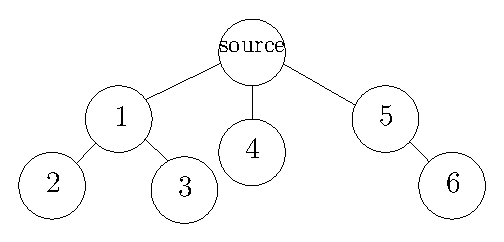
\includegraphics[width=0.3\textwidth]{figures/dfsvisit.eps}
\caption{Example of the visit order in a DFS.}
\end{figure}
\vspace{-12pt}\subsubsection{Graph-based DFS}
\textbf{Pre:} A graph $G=(V,E)$ and a source $S\in V$
\lstinputlisting{code/DFS.java}
\subsubsection{Grid-based DFS}
\textbf{Pre:} A 2D array of nodes and a point $(x,y)$ in the array.
\lstinputlisting{code/DFSGrid.java}

\subsubsection{Connected Components}
\textit{Note: for directed graphs, see Tarjan's (section \ref{sec:tarjan}).}\\
\textbf{Pre:} An undirected graph $G=(V,E)$ and a source $S\in V$.\\
\textbf{Out:} $C$ is the number of components, $\forall_v\ v\in V$, v.component is the 0-based component number of $v$.\\
\textbf{RT:} O($V+E$)
\lstinputlisting{code/DFSConnectedComponents.java}

\subsubsection{Tarjan (Strongly Connected Comp.)}\label{sec:tarjan}
\textit{Note: if you construct a graph by taking SCC's as nodes and insert the edges between distinct SCC's, the resulting graph is a DAG}\\
\textbf{Pre:} A directed graph $G=(V,E)$\\
\textbf{Out:} For every node $u\in V$, \lstinline|V[u].c| is the Strongly Connected Component(SCC) that node is currently in. Two nodes $u,v\in V$ are in the same SCC if and only if $u$ can reach $v$ and  $v$ can reach $u$.\\
\textbf{RT:} O($V+E$)
\lstinputlisting{code/Tarjan.java}

\subsubsection{Topological sort (DAG)}\label{sec:topologicalsort}
\textit{Note: if after this} $\exists u\in V$ : \lstinline|V[u].in != -1|\textit{, then $G$ is cyclic.}\\
\textbf{Pre:} A DAG(= directed, acyclic) $G=(V,E)$\\
\textbf{Out:} \lstinline|ArrayList| of nodes, sorted in topological order.\\
\textbf{RT:} O($V+E$) 
\lstinputlisting{code/DFSTopologicalSort.java}

\subsection{Breadth-first search (BFS)}
\textbf{Pre:} A graph $G=(V,E)$ and a source $S\in V$ with $N=\#V$\\
\textbf{Out:} Visits all $v\in V$ for which $\exists\ $path$($source$, v)$, such that \lstinline|v.visited == true| and \lstinline|v.dist| contains the distance from source to $v$.
\\
\textbf{RT:} O($V+E$)
\vspace{-15pt}
\begin{figure}[H]
\centering
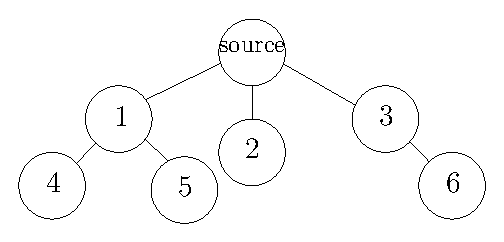
\includegraphics[width=0.3\textwidth]{figures/bfsvisit.eps}
\caption{Example of the visit order in a BFS.}
\end{figure}\vspace{-12pt}
\lstinputlisting{code/BFS.java}

\subsection{Shortest path}
\textit{Note: if all edges have equal weights, you can use a BFS. For each $v\in V$, multiply \lstinline|v.dist| with the weight to get the distance of $v$.}

\textit{In case of a DAG, topological sort (section \ref{sec:topologicalsort}) first, then visit nodes in order and relax all outgoing edges.}
\subsubsection{Dijkstra (single source, positive weight)}
\textbf{Pre:} A weighted graph $G=(V,E)$, where all edges have weight $\geq0$ and a source $S\in V$.\\
\textbf{Out:} For each $v\in V$, \lstinline|v.dist| is the length of the shortest path from source to v and \lstinline|v.parent| is the previous node on that path.\\
\textbf{RT:} O($(V+E)\cdot\log(V))$
\lstinputlisting{code/Dijkstra.java}

\subsubsection{Bellman-Ford (negative weight)}
\textbf{Pre:}  A weighted graph $G=(V,E)$, where $N=\# V$ and a source $S\in V$. Some edges may have negative weight.\\
\textbf{Out:} For each $v\in V$, \lstinline|v.dist| is the length of the shortest path from source to v and \lstinline|v.parent| is the previous node on that path.\\
\textbf{RT:} O($V\cdot E)$
\lstinputlisting{code/BellmanFord.java}
\textbf{Negative weight cycles}\\
If the sum of the weights of all edges in a cycle is negative, you have a negative weight cycle. Computing the shortest path in that case is impossible. To detect if such a cycle is reachable from node source, you can do the following in O($V+E$) time.
\lstinputlisting{code/BellmanFordCycle.java}

\subsubsection{Floyd-Warshall (all pairs shortest path)}
\textbf{Pre:} A weighted graph $G=(V,E)$ where $N=\# V$.\\
\textbf{Out:} $\forall u,v\in V:$ \lstinline|dist[u][v]| is the distance from $u$ to $v$.\\
\textbf{RT:} O($V^3$)
\lstinputlisting{code/FloydWarshall.java}

\subsection{Prim (Minimum Spanning Tree/MST)}
\textbf{Pre:} A weighted undirected graph $G=(V,E)$.\\
\textbf{Out:} A list of NW's, which describe the source, target and weight of the edges in the MST. \lstinline|L2| contains only those edges, \lstinline|L| contains additional edges which are $\not\in E$.\\
\textbf{RT:} O($E\cdot\log(V))$
\lstinputlisting{code/Prim.java}

\subsection{Computing Euler Tour/Path}
\textbf{Pre:} A graph $G=(V,E)$ for which an Euler tour/path is possible and a starting vertex \lstinline|start|. If $G$ undirected, \lstinline|start| can be arbitrary, else \lstinline|start| needs to have odd number of outgoing edges.\\
\textbf{Out:} A \lstinline|L| containing a possible order to visit each edge exactly once. If tour, then start = end. If path, start $\neq$ end. If $G$ doesn't admit an Euler tour/cycle, weird output.\\
\textbf{RT:} O$(V+E)$
\lstinputlisting{code/Euler.java}

\subsection{Maximum Flow}\label{sec:maxflow}
\textit{The} \lstinline|augment()| \textit{method is supplied by either Ford Fulkerson (\ref{alg:ford-fulkerson}), Edmonds Karp (\ref{alg:edmonds-karp}) or Min Cost Flow (\ref{sec:mincostflow})}\\
\textbf{Pre:} A flow network $G=(V,E)$ with a source $s\in V$ and a sink $t\in V$ such that \lstinline|nodes[s]| and \lstinline|nodes[t]| are valid nodes, $N=\#V$\\
\textbf{Out:} The maximum flow $f^*$ of $G$.
\lstinputlisting{code/MaxFlow.java}

\subsubsection{Ford Fulkerson (DFS)}\label{alg:ford-fulkerson}
\textbf{RT:} O($E\cdot f^*$) ($f^*=$ max flow)
\lstinputlisting{code/MaxFlowFordFulkerson.java}

\subsubsection{Edmonds Karp (BFS)}\label{alg:edmonds-karp}
\textbf{RT:} O($V\cdot E^2$)
\lstinputlisting{code/MaxFlowEdmondsKarp.java}

\subsubsection{Minimum Cost Maximum Flow}\label{sec:mincostflow}
\textit{Uses code from section \ref{sec:maxflow}}\\
\textbf{Out:} computes the maximum flow, but will pick the edges in such a way that the total cost is minimized.\\
\textbf{RT:} O($V^2\cdot E^2)$
\lstinputlisting{code/MinCostFlow.java}

\subsection{Bipartite Matching}\label{sec:bipartite_matching}
\textbf{Pre:} Bipartite graph, represented by 2 arrays of nodes; A of length $p$ and B of length $q$. Edges only from A to B, all with weight/capacity 1.\\
\textbf{Out:} $M$, where $M$ is the maximum size set $S\subseteq V$ such that $\forall x\in S : deg(x) = 1$. I.e. create bijective function $F : A \rightarrow B$. Also, if $B[i].match = j$, then node $j\in A$ maps to $i\in B$.\\
\textbf{RT:} O($V\cdot E)$

\lstinputlisting{code/BipartiteMatching.java}
For the \textbf{Minimum Vertex Cover} problem, see section \ref{sec:MinVertexCover}
\subsubsection*{Maximum Independent Set}
\textbf{Problem:} Maximum size set $S\subseteq V$ such that there does not exist an edge between nodes in $S$.\\
\textbf{Solution:} $p+q-M$

%\subsubsection{Maximum weighted bipartite matching}
%\lstinputlisting{code/BipartiteMatchingWeighted.java}

%\section{NP-hard problems}
%\subsection{Traveling Salesman (TSP)}
%\textbf{Pre:} $n$ nodes numbered $0,1,\ldots,n-1$. Distance between nodes is stored in an adjacency array $D[][]$, where $D[i][j]$ contains distance from node $i$ to node $j$.\\
%\textbf{Out:} A shortest tour (start = end) through all nodes. Length is returned. tour[$i$] contains (0-based) the index of the $i$-th node in the tour.\\
%\textbf{RT:} O$((n-1)!)$ maximum (uses pruning)
%\lstinputlisting{code/TSP.java}
\subsection{Useful theorems/lemmas/tricks}
\begin{enumerate}[nolistsep,noitemsep]
\itemsep0em
\item A tree has $V-1=E$
\item A flow network $G_f$ with only integral capacities has integral max flow + all flows for the edges are integral (if you use Ford-Fulkerson/Edmonds Karp)
\item Take a flow network $G_f$ with a cut $(S,T)$, where source $\in S$, sink $\in T$, $V=S\cup T$, $S\cap T=\emptyset$. Then a cut makes it impossible to go from source to sink. The value of a cut is the sum of the capacities of edges from $S$ to $T$(reverse not included). Minimum value of that cut = Max Flow.
\item To check if a graph is a DAG, topological sort it and see if there is no $u\in V$ with $V[u].in\geq 0$. If that is true, then the graph is DAG.
\item To check if a graph is bipartite, start naming vertices either 1 or 2, such that no two vertices connected by an edge have the same name. If this is possible, then the graph is bipartite.
\item To check if a graph admits an Euler tour (start = end), check if every vertex has an even number of edges connected.
\item To check if a graph admits an Euler path (start $\neq$ end), check if every vertex has an even number of edges connected, except for two vertices $u,v$, who needs uneven number of edges. Case directed: $u$ needs one more outgoing edge then there are incoming, $v$ one less. Then, $u$ is start, $v$ is end.
\end{enumerate}

\section{Dynamic Programming (DP)}\label{sec:dp}
\subsection{Knapsack Problem}
\textbf{Pre:} $n,m\in\mathbb{N}\land n,m\geq1$ and an array \lstinline|items[]| of size $n$, containing for each \lstinline|Item i| in \lstinline|items|, \lstinline|i.value| and \lstinline|i.weight| \\
\textbf{Out:} Max value of picking n items with total weight $\leq m$\\
\textbf{RT:} O($m\cdot n$)
\lstinputlisting{code/Knapsack.java}

\subsection{Longest Common Subsequence}
\textbf{Pre:} Char/int/double array A[] of length $P$ and Char/int/double array B[] of length $Q$.\\
\textbf{Out:} Length of longest common subsequence (= sequence that can be obtained by omitting 0 or more characters) of A and B. Get retrieves an ArrayList with the actual sequence. If \lstinline|L = get(P,Q)|, then \lstinline|L.get(0)| is first element of the LCS and \lstinline|L.get(dp[P][Q]-1)| is the last element.\\
\textbf{RT:} O$(P\cdot Q)$ for determining length, O($P+Q$) for \lstinline|get(P,Q)|
\lstinputlisting{code/LongestCommonSubsequence.java}



\subsection{Edit Distance (Difference of Strings)}
\textbf{Pre:} Char array A[] of length $M$ and Char array B[] of length $N$. \lstinline|iC(x)| is a function that calculates the cost of inserting \lstinline|x|. \lstinline|dC(x)| is delete cost for \lstinline|x|. \lstinline|sC(x,y)| is the cost for changing \lstinline|x| into \lstinline|y|.\\
\textbf{Out:} Minimum cost needed to change A into B.\\
\textbf{RT:} O$(M\cdot N)$.
\lstinputlisting{code/EditDistance.java}

\subsection{Coin Counting}
\textbf{Pre:} $n\in\N$ and an array \lstinline|coins[]| specifying for each coin \lstinline|i| its value \lstinline|coins[i]|, where \lstinline|coins[i] > 0| and each value in \lstinline|coins[]| is unique.\\
\textbf{Out:} the number of distinct ways to create the value $n$ using only the coins in \lstinline|coins[]|.\\
\textbf{RT:} O($n^2)$
\lstinputlisting{code/CoinCountDP.java}

\subsection{Coin Change}
\textbf{Pre:} $n\in\N$ and an array \lstinline|coins[]| specifying for each coin \lstinline|i| its value \lstinline|coins[i]|, where \lstinline|coins[i] > 0| and each value in \lstinline|coins[]| is unique.\\
\textbf{Out:} the minimum number of coins needed to create \lstinline|n| from \lstinline|coins|, where \lstinline|R| contains the actual coins used to form \lstinline|n|.\\
\textbf{RT:} O($n^2)$
\lstinputlisting{code/CoinChange.java}

\subsection{Subset DP}
\textit{Note: this makes use of bitmasks (section \ref{sec:bitmask})}\\
This is a technique for solving problems. Use it when it looks like a DP problem, but the solution depends on which subset of things you already have. The number of elements in the set should be small $(\leq 16)$. Also consider applying memoization, especially for multiple dimensions.
\section{Miscellaneous Stuff}
%\subsection{Binary Search}
%\textbf{Pre:} Sorted array E[] A of length $N$ and a key of type E.\\
%\textbf{Out:} $-1$ if key $\not\in A$, else an index of key in A.\\
%\textbf{RT:} O($\log(N)$)
%\lstinputlisting{code/BinarySearch.java}

\subsection{String Matching (KMP)}
\textbf{Pre:} \lstinline|char[] pattern| of size $m$ and \lstinline|char[] text| of size $n$.\\
\textbf{Out:} All indexes where pattern occurs in text.\\
\textbf{RT:} O($n+m$)
\lstinputlisting{code/KMP.java}

\subsection{Longest Increasing Subsequence}
\textbf{Pre:} An array of integers \lstinline|A| with \lstinline|n = A.length;|\\
\textbf{Out:} \lstinline|ans| contains the elements of the longest \textit{strictly} increasing subsequence, where \lstinline|ans.size() = length + 1|.\\
\textbf{RT:} O($n\log(n))$\\
\textbf{Example:} \lstinline|A = {3,4,-1,5,8,2,3,12,7,9,10,10};|. Then, 
\\\lstinline|n = 12;| and a possible LIS \lstinline|= {-1,2,3,7,9,10};| Note that there does not exist a longer one.
\lstinputlisting{code/LongestIncreasingSubsequence.java}

\subsection{Impartial Game Theory}
\textbf{Identifiers of an impartial game:}
\begin{enumerate}[nolistsep,noitemsep,label*=\arabic*.]
\itemsep0em
\item Two player game where moves are (usually) alternated
\item No simultaneous moves are allowed
\item For every state specified which moves are legal
\item Game ends when no move is possible in a turn
\begin{enumerate}[nolistsep,noitemsep,label*=\arabic*.]
\item Normal play rule: last player to move wins
\item Mis\`ere play rule: last player to move loses (hard)
\end{enumerate}
\item No draws are allowed
\item Game always has a finite number of moves
\item Both players have the same set of moves available. So, legal set of moves only depends current state, not which of the two players is moving
\end{enumerate}
\textbf{Labeling states with P/N:}\\
First create a graph where nodes represent legal states and edges represent legal moves. Label states with P(revious) if it secures a win for the player who has just moved. Label states with N(ext) if it secures a win for the player about to make a move. Generally, final states are P (normal play rule). If dealing with objects on a pile, state with 0 items on pile is final state.

For nodes which have not been determined: label with P if all next nodes are N. If at least one moves leads to a P node, label it N. If initial state is N, first player to moves can win, else the other player. Strategy is to make moves leading to P nodes.
\subsubsection{Sprague-Grundy Function}
The \textbf{mex} of a set is the smallest value $(\geq0)$ not contained in the set. Some examples:
\begin{itemize}[nolistsep,noitemsep]
\itemsep0em
\item $mex(\emptyset) = 0$ (often the final state)
\item $mex(\{1, 2, 3\}) = 0$
\item $mex(\{0, 2, 4, 6, ...\}) = 1$
\item $mex(\{0, 1, 2, 4, 5\}) = 3$
\end{itemize}
Function: $G(v) = mex(\{G(w)$ if $(v,w)\in E\})$. Generally, if $G(v)=0$, the state is P. If bigger, then the state is N. 

In case of multiple games forming one game, for every subgame, calculate its $G(v)$ value and take the XOR of all those values.

\section{Rare Problems and Solutions}
\subsection{Traveling Salesman Problem (TSP)}
\textbf{Problem:} Given a set of $n$ cities $0,\ldots,n-1$ and for every pair of cities $(i,j)$ the distance between them, \lstinline|dist(i, j)|, what is the shortest cycle visiting every city exactly once?\\
\textbf{Solution:} O($n^2\cdot2^n)$ Subset DP. Create a 2D array \\\lstinline|int[n][(1<<n)] dp|. The solution will be in \lstinline|dp[0][1]|.\\
\lstinline|dp[i][j] = dist(i,0)|\hspace{6pt} if \lstinline|i == (1<<n)|\\
\lstinline*dp[i][j] = min{dist(i,nxt)+dp[nxt][j|(1<<nxt)]}*
\\\tab $\forall_{nxt}\ 0\leq$ \lstinline|nxt| $<n\ \land$ \lstinline|nxt| $\neq$ \lstinline|j| $\land$ \lstinline|(j & (1 << nxt))| $=0$

\subsection{Bitonic TSP}
\textbf{Problem:} Given a set of $n$ points on a 2D plane. What is the shortest cycle starting at the leftmost point, moving onl to the right and when at the rightmost point moving only to the left.\\
\textbf{Solution:} O($n^2$) Dynamic Programming. Sort all points by x-coordinate (leftmost point with index 0, rightmost point with index $n-1$). Create a 2D array \lstinline|int[n-1][n-1] dp| and solve it using the recurrence below. Finally, compute the solution as follows: \\$dp[n-1][n-1] = min_{0\leq k<n-1}\{dp[n-1,k]+dist(k,n-1)\}$\vspace{-5pt}
\[
      dp[i,j] = \left\{
                   \begin{array}{ll}
                     dist(0,1) & \mbox{if $i=1\land j=0$} \\
                     dp[i-1,j]+dist(i-1,i) & \mbox{if $(i-1)>j$} \\
                     min_{0\leq k<j}\{dp[j][k]+dist(k,i)\} & \mbox{if $(i-1) = j$} \\
                   \end{array}
                \right.
      \]
\subsection{2-Satisfiability (2SAT)}
\textbf{Problem:} Given a boolean formula of the following form: $F=(x_1\lor\lnot x_2) \land(\lnot x_1\lor\lnot x_3)\land(x_2\lor x_4)$, is there a true/false assignment to the variables such that $F$ yields true.\\
\textbf{Solution:} Create a directed graph. For each variable, create two nodes, $a$ and $\lnot a$. Then, for every $(a\lor b)$, add an edge from $\lnot a$ to $b$ and from $\lnot b$ to $a$. Then, run Tarjan's algorithm (see section \ref{sec:tarjan}). For every SCC, check for every variable if $a$ and $\lnot a$ are present. If so, it is not possible.

To compute the actual assignment, turn each SCC into one node. New graph is a DAG. Topologically sort the nodes (see section \ref{sec:topologicalsort}). Visit SCC's in reverse topological order. Set all variables in last SCC to true. In all complementary SCC's (which contains $a$, whilst $\lnot a$ has been determined), turn every variable to the complementary value.

\subsection{Bracket Matching}
\textbf{Problem:} Given a set of brackets: ()\{[\}])(, does it follow a standard bracket structure (e.g. ()([()]) )\\
\textbf{Solution:} O($n)$. Push every opening bracket on top of a \lstinline|Stack<B>| (or \lstinline|ArrayDeque|, section \ref{sec:LinkedList/ArrayDeque}). For closing brackets, poll the topmost element from the stack and see if it matches. If all match, it is valid.
\subsection{Minimum Vertex Cover} \label{sec:MinVertexCover}
\textbf{Problem:} NP-hard. Given a graph $G$, what is the minimum number that you can select such that each edge is touched by at least one selected vertex. (Or: what is the minimum number of vertices to remove such that every edge gets removed).\\
\textbf{Solution:} O($2^n)$ brute force. For every edge, recurse with two possible options: remove left node (and all connected edges) or remove right node (and all connected edges).

If the graph is bipartite, you can use Bipartite Matching (section \ref{sec:bipartite_matching}) and return $M$.

\subsection{Stable Marriage}
\textbf{Problem:} Given two disjoint sets of the same size, $A$ and $B$, where each element of $A$ has rated how much they want to be paired up with each element of $B$ and vice versa, where no element has rated two other elements the same. What is the best possible matching such that each element from $A$ is paired with an element from $B$ and that it is not possible for one of the two to find another element such that both elements in the new pair are happier.\\
\textbf{Solution:} O($n^2$). For each element in $A$, let them pick the element they have ranked highest. Each element in $B$ always accepts. If an element in $B$ has multiple elements to choose from, it chooses the one it ranked highest. If it has already picked an element, it can drop it for a new element which it ranked higher. Repeat until done.
\end{multicols}
\end{document}